\documentclass[11pt]{ltjsarticle}
\usepackage[margin=25mm]{geometry}
\usepackage{amsmath,amssymb,amsthm}
\usepackage{booktabs}
\usepackage{graphicx}
\usepackage{tikz}
\usetikzlibrary{arrows.meta,positioning,shapes.geometric,calc}
\usepackage{hyperref}

\newtheorem{proposition}{命題}
\newtheorem{lemma}{補題}
\newtheorem{remark}{注意}
\newtheorem{definition}{定義}

\DeclareMathOperator*{\argmin}{arg\,min}

% u64 wrapping (mod 2^64) 演算子
\newcommand{\wadd}{\mathbin{\boxplus}}
\newcommand{\wmul}{\mathbin{\boxdot}}
% 大型 wrapping 総和（添字は下付き）
\newcommand{\bigwadd}{\mathop{\scalebox{1.45}{$\boxplus$}}}
\newcommand{\idx}{\mathrm{idx}}
\newcommand{\Rmax}{R_{\max}}        % 原論文の番兵 R_max
\newcommand{\Cfree}{\mathcal{C}_{\mathrm{free}}}
\newcommand{\Cocc}{\mathcal{C}_{\mathrm{occ}}}
\newcommand{\Cnear}{\mathcal{C}_{\mathrm{near}}}
\newcommand{\Xgoal}{\mathcal{X}_{\mathrm{goal}}}

\title{価値反復ソルバ \texttt{reference} の数式モデル\\\large——u64 固定小数点上の確率的最短経路}
\author{ソルバ仕様ノート}
\date{2026-06}

\begin{document}
\maketitle

\begin{abstract}
本ノートは、向きを含む格子地図上の経路計画を解く価値反復ソルバ \texttt{reference} の計算を数式で
定義する。対象は Ueda ら (2023) の brute-force value iteration\footnote{R. Ueda, L. Tonouchi, T. Ikebe,
and Y. Hayashibara, ``Implementation of Brute-Force Value Iteration for Mobile Robot Path Planning and
Obstacle Bypassing,'' \textit{J. Robot. Mechatron.}, Vol.35, No.6, pp.~1489--1502, 2023.}
を $64$ ビット整数の固定小数点で実装したもので、記法・変数記号も可能な範囲で同論文に合わせる（要所で
原論文の式番号を併記する）。状態空間・固定小数点表現・確率遷移・ステップコスト・Bellman 更新・ゴール処理を
順に与え、この問題が\emph{割引なし確率的最短経路（SSP）}にあたることを示して、各状態の最適コスト
（cost-to-go）を表す固定点が到達可能な範囲で一意に定まることを述べる。最後に整数演算ゆえに結果へ影響する
数値的性質を補足する。ここで定める更新式は、同じ式を一部の状態だけに速く適用する各種高速ソルバの基準
（収束値の照合元）となる。
\end{abstract}

\tableofcontents

\section{問題設定}
\label{sec:setup}

移動ロボットの経路計画を、平面位置 $(x,y)$ と向き $\theta$ を離散化した格子の上で考える。各状態
$s=(i_x,i_y,i_\theta)$ について、そこからゴールに到達するまでに要するコストの期待値、すなわち
\textbf{cost-to-go}（ゴールまでの期待コスト、単位は秒）を値 $V(s)$ として求め、同時に各状態で取るべき
最適な行動 $a^\ast=\pi(s)$ を決めるのが目的である。ロボットの制御入力は並進速度 $\nu$ と回転速度 $\omega$ の
組 $u=(\nu,\omega)$ で、これを離散化した有限個の\textbf{行動} $a\in\mathcal{A}$ から選ぶ。行動は確率的に
隣の状態へ遷移する。

価値反復（value iteration）は、$1$ つの更新規則である\textbf{Bellman 更新}を全状態に繰り返し適用して $V$
を改善し、それ以上変化しなくなった\textbf{固定点} $V^\star$ を解とする動的計画法である。本ノートは、この
更新を $64$ ビット整数（u64）上の固定小数点で実装した基準ソルバ \texttt{reference} の計算を、厳密に書き
下す。

\section{記法と定数}
\label{sec:notation}

格子は $N_x\times N_y\times N_\theta$ の状態からなり、状態数は $N_s=N_x N_y N_\theta$。平面の $1$ マスを
\emph{セル} $c=(i_x,i_y)$ と呼び、各セルに $N_\theta$ 通りの向き $i_\theta$ を積んだものが状態空間
$\mathcal{S}$ である（図~\ref{fig:arrays}）。配列上の位置を一意に表すフラット索引を
\begin{equation}
\idx(s) \;=\; i_\theta + i_x\,N_\theta + i_y\,N_\theta N_x
\label{eq:idx}
\end{equation}
とする（$\theta$ を最内、次に $x$、最外に $y$ を並べる。原論文 Eq.~(17) の $1$ 始まり版に対応する）。

\begin{figure}[h]
\centering
\begin{tikzpicture}[scale=0.95, every node/.style={font=\small}]
  \def\px{3.4}\def\sx{1.0}\def\sy{0.55}
  % occupancy grid (bottom)
  \draw[fill=black!12] (0,0) -- (\px,0) -- (\px+\sx,\sy) -- (\sx,\sy) -- cycle;
  \node[anchor=west] at (\px+\sx+0.3,0.28) {占有格子地図（白＝自由 / 黒＝障害）};
  % cost map
  \begin{scope}[shift={(0,1.05)}]
   \draw[fill=orange!20] (0,0) -- (\px,0) -- (\px+\sx,\sy) -- (\sx,\sy) -- cycle;
   \node[anchor=west] at (\px+\sx+0.3,0.28) {コストマップ $r'(c)$};
  \end{scope}
  % value layers (stack of N_theta)
  \foreach \i in {0,1,2,3} {
   \begin{scope}[shift={(0,2.2+\i*0.24)}]
    \draw[fill=blue!10] (0,0) -- (\px,0) -- (\px+\sx,\sy) -- (\sx,\sy) -- cycle;
   \end{scope}
  }
  \node[anchor=west] at (\px+\sx+0.3,2.95) {値 $V$（向きごとに $N_\theta$ 層）};
  \draw[-{Stealth}] (\px+\sx+0.05,0.7) to[out=90,in=270] (\px+\sx+0.05,2.1);
\end{tikzpicture}
\caption{データ配列。$2$ 次元の占有格子地図とコストマップに向き $\theta$ の軸を加え、$N_\theta$ 枚の層を
積んだ $3$ 次元配列が状態空間 $\mathcal{S}$ になる。}
\label{fig:arrays}
\end{figure}

値とコストはすべて u64 上の\textbf{固定小数点}で表す。これは価値反復を整数演算だけで実行するための
工夫で、下位 $b_B=18$ ビットを小数部に使う。したがって整数 $B=2^{18}$ が実数の $1.0$ にあたり、$1$ 歩
（$\Delta t=1$ 秒）のコストはちょうど $B$ になる。主要な定数を表~\ref{tab:const} に示す。番兵値は原論文と
同じく $\Rmax$ と書き、「まだ値が伝わっていない／到達できない」状態と、占有セルの値を表す。

\begin{table}[h]
\centering
\begin{tabular}{llr}
\toprule
記号 & 意味 & 値 \\
\midrule
$b_B$    & 小数部ビット数 & $18$ \\
$B$      & 実数 $1.0$ にあたる整数 $=2^{b_B}$（$1$ 歩のコスト） & $262{,}144$ \\
$\Rmax$  & 番兵（未到達・占有）$=10^{9}\,B$ & $262{,}144{,}000{,}000{,}000$ \\
$K$      & 各軸のサブセル分割数 $=2^{6}$ & $64$ \\
\bottomrule
\end{tabular}
\caption{固定小数点定数。$\Rmax$ は原論文 Eq.~(6),(12) の $R_{\max}$ にあたる。}
\label{tab:const}
\end{table}

各状態は値 $V(s)$ と二つのペナルティ $\rho(s)$（静的）・$\lambda(s)$（動的）を持つ。自由（通行可能）な状態
の集合を $\mathcal{F}$、ゴールの集合を $\Xgoal\subseteq\mathcal{F}$ と書く（\S\ref{sec:goal}）。整数演算では
桁あふれが起こり得るため、$2^{64}$ で割った余りに丸める加算・乗算（wrapping 演算）を $\wadd,\wmul$、整数
右シフト（$=\lfloor\cdot/2^{k}\rfloor$）を $\gg k$ と書く。

行動の集合 $\mathcal{A}$ は、制御入力 $(\nu,\omega)$ を離散化した $6$ 種からなる（表~\ref{tab:actions}、
原論文 Table~1 と同じ）。$1$ ステップ（$\Delta t$ 秒）の並進距離は $\ell_a=\nu_a\Delta t$、回転は
$\Delta\theta_a=\omega_a\Delta t$ である。

\begin{table}[h]
\centering
\begin{tabular}{lrr}
\toprule
行動 & $\nu$ [m/s] & $\omega$ [$^\circ$/s] \\
\midrule
前進 (forward)        & $0.3$  & $0$   \\
後退 (backward)       & $-0.2$ & $0$   \\
右回転 (right)        & $0.0$  & $-20$ \\
右前進 (right forward)& $0.2$  & $-20$ \\
左回転 (left)         & $0.0$  & $+20$ \\
左前進 (left forward) & $0.2$  & $+20$ \\
\bottomrule
\end{tabular}
\caption{行動集合（並進速度 $\nu$・回転速度 $\omega$）。$\Delta t=1$ 秒。}
\label{tab:actions}
\end{table}

\section{確率遷移モデル}
\label{sec:trans}

同じ行動を選んでも、源セル内のどこにいたかによって着地するセルはばらつく。原論文はこの\textbf{状態遷移
確率} $P(s'\,|\,s,a)$ を、相対変位 $\Delta s'$ の確率 $P(\Delta s'\,|\,i_\theta,a)$ として\textbf{モンテ
カルロ積分}で求める（原論文 Eq.~(10),(11)）。実装は積分を、各セルを $K\times K\times K=K^3$ 個の小領域
（サブセル）に分け、各サブセル中心を運動モデルで飛ばして着地セルを数え上げるサンプリングで行う
（図~\ref{fig:mc}）。以下その手続きを述べる。

\begin{figure}[h]
\centering
\begin{tikzpicture}[scale=0.85, every node/.style={font=\small}, >={Stealth}]
  \draw[step=1, gray!45, thin] (0,0) grid (3,3);
  % source cell subdivided
  \draw[step=0.25, gray!40, very thin] (1,1) grid (2,2);
  \draw[thick] (1,1) rectangle (2,2);
  \node[below] at (1.5,1.0) {源セル};
  \foreach \x in {1.125,1.375,1.625,1.875}
    \foreach \y in {1.125,1.375,1.625,1.875}
      \fill[blue!55] (\x,\y) circle (0.5pt);
  % arrows to neighbours, thickness ~ probability
  \draw[->, line width=1.6pt] (1.75,1.75) -- (2.55,2.45);
  \draw[->, line width=1.0pt] (1.8,1.5) -- (2.6,1.5);
  \draw[->, line width=0.5pt] (1.5,1.8) -- (1.5,2.55);
  \node[anchor=west] at (3.2,1.5) {相対遷移確率 $P(\Delta s'\,|\,i_\theta,a)$};
\end{tikzpicture}
\caption{モンテカルロ積分。源セルを $K^3$ 個のサブセルに分け、各中心を運動モデルで飛ばして着地セルを数え、
相対変位ごとの確率を得る。矢印の太さは確率の大小を表す。}
\label{fig:mc}
\end{figure}

まず、空間解像度を $\Delta_{xy}$ [m]、角度解像度を
\begin{equation}
\Delta_t \;=\; \big\lfloor 360/N_\theta\big\rfloor \quad[\mathrm{deg}]
\label{eq:tres}
\end{equation}
とする（\eqref{eq:tres} は整数除算。注意~\ref{rem:intdiv}）。サブセルの刻みは
$h_{xy}=\Delta_{xy}/K,\ h_t=\Delta_t/K$、その中心は
$o^{x}_{k}=o^{y}_{k}=(k+\tfrac12)h_{xy}$、$o^{t}_{k}=(k+\tfrac12)h_t$（$k=0,\dots,K-1$）に置く。

次に、源の角度インデックス $t=i_\theta$ の原点角を $\theta_0=t\,\Delta_t$ [deg]、サブセル
$(o^x,o^y,o^t)$ の見出し角を $\beta=(\theta_0+o^t)\,\pi/180$ として、運動後の連続的な着地点を
\begin{equation}
x'=o^x+\ell_a\cos\beta,\qquad
y'=o^y+\ell_a\sin\beta,\qquad
\theta'=\theta_0+o^t+\Delta\theta_a
\label{eq:cont}
\end{equation}
で求める（$\ell_a=\nu_a\Delta t$、$\Delta\theta_a=\omega_a\Delta t$）。ここで $\theta'$ は $\theta'<0$ の
ときだけ $+360$ して正の範囲に直す（$\theta'\ge360$ はそのまま。注意~\ref{rem:theta}）。

最後に、連続点 $(x',y',\theta')$ をセル単位の相対変位 $\Delta s'=(d_{ix},d_{iy},d_{it})$ に量子化する：
\begin{equation}
d_{ix}=
\begin{cases}
\big\lfloor |x'|/\Delta_{xy}\big\rfloor & x'\ge 0\\[2pt]
-\big\lfloor |x'|/\Delta_{xy}\big\rfloor-1 & x'<0
\end{cases}
\qquad
d_{it}=\big\lfloor \theta'/\Delta_t\big\rfloor
\label{eq:celldelta}
\end{equation}
（$d_{iy}$ は $d_{ix}$ と同じ形）。ここで $d_{it}$ は源の $i_\theta$ を含んだ\textbf{絶対}の角度インデックス
で、この段階では $N_\theta$ の余りをとらない点に注意する。

以上を $(a,t)$ ごとに $K^3$ サンプル集計すると、相対遷移確率が整数の重み付き分布
\begin{equation}
\big\{(\Delta s',\,p)\big\}=P(\Delta s'\,|\,i_\theta{=}t,\,a),\qquad
p=(\text{$\Delta s'$ に着地したサブセル数}),\qquad
\sum p \;=\; K^3 \;=\; B
\label{eq:tau}
\end{equation}
として得られる。重みの総和がちょうどスケール $B$ になるので、確率は $P=p/B$ で表せる。直感的には、前進系の
行動は主に空間方向へ、回転系の行動（$d_{ix}=d_{iy}=0$）は角度方向へ分布が広がる。

\section{ステップコスト（コストマップ）}
\label{sec:cost}

行動の良し悪しは $1$ ステップに要する時間で測る。原論文の評価関数（Eq.~(3)）は
\begin{equation}
r(s)\;=\;\Delta t\,\{1+r'(c)\}
\label{eq:r}
\end{equation}
で、$\Delta t$ は $1$ ステップの時間、$r'(c)$ は\textbf{コストマップ}（走りにくさ。ROS のコストマップに相当）
である。コストマップは、占有・未知セル $\Cocc$ とその近傍 $\Cnear$ で大きく、自由セル $\Cfree$ で $0$ に
初期化される（原論文 Eq.~(6)）。固定小数点では $\Delta t\cdot1=B$ なので、$1$ 歩の基本コストが $B$、
コストマップぶんが上乗せになる。実装ではこれを静的ペナルティ
\begin{equation}
\rho(s)\;=\;B\wadd\big\lfloor r'(c)\,B\big\rfloor=
\begin{cases}
B & \text{障害物から離れた自由セル }(r'{=}0),\\
\big\lfloor c_{\mathrm{pen}}\,B\big\rfloor + B & \text{安全マージン内の自由セル }(r'{=}c_{\mathrm{pen}}{>}0)
\end{cases}
\label{eq:penalty}
\end{equation}
として持つ（$c_{\mathrm{pen}}$ はマージン侵入の重み。探索範囲は注意~\ref{rem:margin}）。占有セルは通行不可
として扱い、参照されると番兵 $\Rmax$ を返す（\S\ref{sec:bellman}）。動的ペナルティ $\lambda(s)$ は、センサ
で見つかった一時障害物を反映する分（原論文の局所窓更新 Eq.~(8),(9)、減衰率 $\gamma$）で、本ノートが扱う
静的計画では $\lambda\equiv0$ とする。$1$ 歩あたり必ず加わるステップコストを
\begin{equation}
r(s)\;=\;\rho(s)\wadd\lambda(s)\;\ge\;B\;>\;0
\label{eq:g}
\end{equation}
とまとめる（\eqref{eq:r} を固定小数点で実体化したもの）。$r$ が厳に正であることは、後述する解の一意性
（\S\ref{sec:goal}）の鍵になる。

\section{行動コストと Bellman 更新}
\label{sec:bellman}

\paragraph{Bellman 更新（概念）。}
状態 $s$ で行動 $a$ を選ぶコストは、遷移先 $s'$ の「値 $+$ ステップコスト」を確率で重み付き平均した
ものである。各状態では、それを最小にする行動を選ぶ（図~\ref{fig:bellman}）。これが原論文 Eq.~(13) の
Bellman 更新である：
\begin{equation}
V(s)\;\leftarrow\;\min_{a\in\mathcal{A}}\ \sum_{s'\in\mathcal{S}} P(s'\,|\,s,a)\,\big\{V(s')+r(s')\big\}.
\label{eq:bellman13}
\end{equation}

\begin{figure}[h]
\centering
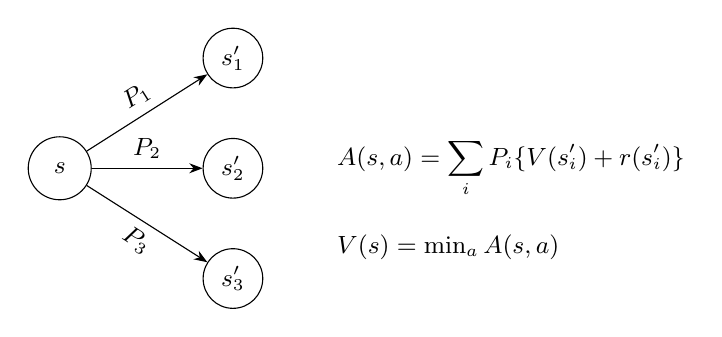
\begin{tikzpicture}[every node/.style={font=\small}, >={Stealth}, node distance=8mm]
  \node[draw,circle,minimum size=8mm] (s) at (0,0) {$s$};
  \node[draw,circle,minimum size=7mm] (a) at (2.2,1.4) {$s'_1$};
  \node[draw,circle,minimum size=7mm] (b) at (2.2,0)   {$s'_2$};
  \node[draw,circle,minimum size=7mm] (c) at (2.2,-1.4){$s'_3$};
  \draw[->] (s) -- (a) node[midway,sloped,above] {$P_1$};
  \draw[->] (s) -- (b) node[midway,above] {$P_2$};
  \draw[->] (s) -- (c) node[midway,sloped,below] {$P_3$};
  \node[anchor=west] at (3.4,0) {$\displaystyle A(s,a)=\sum_i P_i\{V(s'_i)+r(s'_i)\}$};
  \node[anchor=west] at (3.4,-1.0) {$V(s)=\min_a A(s,a)$};
\end{tikzpicture}
\caption{Bellman 更新。行動 $a$ のコスト $A(s,a)$ は遷移先の「値 $+$ ステップコスト」を確率で平均した
もので、全行動で最小をとる。}
\label{fig:bellman}
\end{figure}

\paragraph{固定小数点での実体。}
セル $s$ から相対変位 $\Delta s'$ で移った先を
\begin{equation}
s\oplus\Delta s' \;=\;\big(i_x+d_{ix},\; i_y+d_{iy},\; d_{it}\bmod N_\theta\big)
\label{eq:oplus}
\end{equation}
と書く（角度はここで初めて $N_\theta$ の余りをとる）。確率は $P=p/B$、ステップコストは \eqref{eq:g} の
$r(s')$ なので、\eqref{eq:bellman13} の行動コストは整数演算で次のように評価される。途中いずれかの遷移先が
\emph{範囲外または通行不可}なら、その行動は使えないものとして番兵 $\Rmax$ を返す：
\begin{equation}
A(s,a)=
\begin{cases}
\Rmax, & \exists(\Delta s',p):\ s\oplus\Delta s'\notin\mathcal{F},\\[4pt]
\displaystyle\Big(\;\bigwadd_{(\Delta s',p)}\!\!\big[V(s\oplus\Delta s')\wadd r(s\oplus\Delta s')\big]\wmul p\;\Big)\gg b_B, & \text{それ以外.}
\end{cases}
\label{eq:actioncost}
\end{equation}
重み $p$ の総和が $B$ なので、最後の $\gg b_B$（$=\lfloor\cdot/B\rfloor$）が「確率で割って平均に直す」役目を
果たす（整数除算。注意~\ref{rem:intdiv}）。$\mathcal{F}$ は自由（通行可能）な状態の集合である。Bellman 更新は
$(\mathcal{T}V)(s)=\min_a A(s,a)$、最適行動は $a^\ast=\pi(s)=\argmin_a A(s,a)$（原論文 Eq.~(5)）で、全行動が
$\Rmax$ なら $V(s)=\Rmax$・$\pi(s)=\bot$（未定義）。通行不可セルとゴールでは更新しない。価値反復とは、この
固定点 $V^\star=\mathcal{T}V^\star$ を求めることに他ならない。

\section{ゴール処理と SSP としての定式化}
\label{sec:goal}

\paragraph{ゴール集合。}
ゴール姿勢を $\mathbf{x}_{\mathrm{goal}}=(x_g,y_g,\theta_g)$、許容する距離マージンを $r_{\mathrm g}$
（実験では $300$ mm）、角度マージンを $m_\theta$（実験では $\pm15^\circ$）とする。状態 $s$ がゴールと
みなされるのは、セルの左下角 $(x_0,y_0)$ と右上角 $(x_1,y_1)=(x_0+\Delta_{xy},y_0+\Delta_{xy})$ の両方が
ゴール半径に入り、かつ向きが合い、かつ通行可能なときである：
\begin{equation}
s\in\Xgoal\iff
\underbrace{(x_0-x_g)^2+(y_0-y_g)^2<r_{\mathrm g}^2}_{\text{近い角}}\ \wedge\
\underbrace{(x_1-x_g)^2+(y_1-y_g)^2<r_{\mathrm g}^2}_{\text{遠い角}}\ \wedge\
s\in\mathcal{F}\ \wedge\ \Phi_\theta(s).
\label{eq:goal}
\end{equation}
向き条件 $\Phi_\theta(s)$ は、セルの角度区間
$[t_0,t_1]=[\lfloor i_\theta\Delta_t\rfloor,\lfloor(i_\theta{+}1)\Delta_t\rfloor]$ がゴール角
$\theta_g$（または $360$ 補角）の $\pm m_\theta$ 帯に収まることを表す。初期値は原論文 Eq.~(12)
と同じく
\begin{equation}
V_0(s)=
\begin{cases}
0 & s\in\Xgoal,\\
\Rmax & \text{それ以外}
\end{cases}
\label{eq:init}
\end{equation}
とする。ゴールは値 $0$ のまま更新されない吸収点で、隣のセルがゴールを参照すると $V=0$ にゴール自身の
$r\ge B$ が足されるので、ゴールに着く $1$ 歩も \eqref{eq:actioncost} どおり正のコストを持つ。よってゴールを
特別扱いする必要はない。

\paragraph{SSP としての一意性。}
\eqref{eq:bellman13} は\textbf{割引なし確率的最短経路（SSP）}、すなわち「各ステップに正のコスト $r$ が
かかり、吸収ゴールに着くまでの総コストの期待値を最小化する問題」にあたる。この構造から次が従う。

\begin{proposition}[到達可能な状態で固定点は一意]
\label{prop:unique}
ゴールへ確率 $1$ で到達する方策（proper policy）が存在し、かつ全ステップコストが $r>0$ であるなら、
固定点 $V^\star$ は\emph{到達可能な状態の上で一意}に定まり、価値反復 $V_{k+1}=\mathcal{T}V_k$ は初期値
\eqref{eq:init} からそこへ収束する。
\end{proposition}

\noindent
到達できない状態は値が $\Rmax$ 付近に留まり、$\Rmax\wmul p$ が桁あふれして振動することもある
（注意~\ref{rem:wrap}）が、これは到達可能な状態の解には影響しない。実装上は $V(s)<10^{6}B$ を「到達可能」の
判定に用いる。

\section{求解：Gauss--Seidel スイープ}
\label{sec:solve}

基準ソルバ \texttt{reference} は、Bellman 更新 \eqref{eq:bellman13} を全状態へ繰り返し適用するだけの素直な
実装である。あらかじめ決めた走査順 $\sigma$（既定は $y,x,\theta$ の順）で状態をたどり、各状態の値を
\textbf{その場で}書き換える。更新を即座に書き戻すので、同じ走査内で先に更新した状態の新しい値を後続が読む。
これを\textbf{Gauss--Seidel}（逐次更新）と呼ぶ。この $1$ 巡を $1$ \textbf{スイープ}と数え、$1$ スイープで
到達可能な状態（$V<10^{6}B$）の値が一つも変わらなくなったら収束とみなして停止する。

\begin{figure}[h]
\centering
\begin{tikzpicture}[scale=0.9, every node/.style={font=\small}, >={Stealth}]
  \node[star, star points=5, star point ratio=2.2, fill=red!75, inner sep=1.6pt] at (0,0) {};
  \foreach \rr in {0.75,1.35,1.95,2.55} \draw[gray!70] (0,0) circle (\rr);
  \node[below] at (0,-0.35) {ゴール};
  \node at (0.95,0.0) {\scriptsize $1$};
  \node at (1.55,0.0) {\scriptsize $2$};
  \node at (2.15,0.0) {\scriptsize $3$};
  \draw[->, thick] (0.35,0.3) -- (2.2,1.55) node[right] {$1$ スイープ $=$ $1$ 歩ぶん伝播};
\end{tikzpicture}
\caption{値の伝播。値はゴールから $1$ スイープにつき行動 $1$ 歩ぶんしか広がらない。等高線の数字は確定した
値（歩数）を表す。}
\label{fig:wavefront}
\end{figure}

\paragraph{計算量。}
図~\ref{fig:wavefront} のとおり、ある状態 $s'$ の値の変化は、次のスイープで $P(s'|s,a)\neq0$ となる手前の
状態 $s$ へ伝わる。したがって収束に必要なスイープ数は、原論文が述べるとおり\emph{課題に必要な状態遷移数の
最大}（ゴールからの行動ステップで測った地図の直径 $\mathrm{diam}$）にほぼ比例する。全状態を走査するこの
brute-force な反復は、\emph{すべての状態について最適コストを厳密に求められる}という強みと引き換えに、
\begin{equation}
O(\mathrm{diam}\cdot N_s)
\end{equation}
の計算量をもつ（原論文も計算コストの高さを率直に論じている）。地図が横長になるほど直径が伸び、この計算量が
効いてくる。後段で扱う高速ソルバ、すなわち値が変わる状態だけを追う活性集合（フロンティア）法や、値の小さい
順に状態を確定する優先順序伝播は、この厳密解を保ったまま直径依存の計算量だけを削る。いずれも Bellman 更新を
\emph{状態単位では同じ式}で適用するので、Proposition~\ref{prop:unique} の一意性により収束値は本ソルバと
完全に一致する。

\section{数値的性質}
\label{sec:remarks}

以下は、本アルゴリズムが固定小数点 u64 の上で動くことから生じ、結果に影響する性質である。

\begin{remark}[整数除算による切り捨て]
\label{rem:intdiv}
\eqref{eq:actioncost} 末尾の $\gg b_B$ は $\lfloor\cdot/B\rfloor$ の切り捨てであり、角度解像度
\eqref{eq:tres} $\Delta_t=\lfloor360/N_\theta\rfloor$ も整数除算である。値を $V/B$ で書き出すときも床関数で
丸める。これらの端数切り捨ては全ソルバで共通して起こる。
\end{remark}

\begin{remark}[桁あふれの折り返し]
\label{rem:wrap}
\eqref{eq:actioncost} の総和と乗算は $2^{64}$ で割った余りに丸める。未到達状態（$V=\Rmax$）の近くでは
$\Rmax\wmul p$ が桁あふれして折り返り、$\Rmax$ より小さい値に振動することがある。これは到達可能な状態の解
には影響しないが、値の大小で早期打ち切りを行う近似ソルバでは注意が必要である。
\end{remark}

\begin{remark}[角度の片側だけの正規化]
\label{rem:theta}
\eqref{eq:cont} の $\theta'$ は負のときだけ $+360$ で正規化し、$360$ 以上はそのまま残す。よって
$d_{it}$ \eqref{eq:celldelta} は $[0,2N_\theta)$ の値を取り得て、隣接写像 \eqref{eq:oplus} で初めて
$N_\theta$ の余りに畳まれる。
\end{remark}

\begin{remark}[マージン探索の行またぎ]
\label{rem:margin}
\eqref{eq:penalty} の障害物探索は、二次元の列範囲ではなく\emph{一次元のフラット索引}の境界
（$0\le pos<\text{セル総数}$）だけで内外を判定する。このため左端のセル（$i_x=0$）で $i_x-1$ を見ると、
索引が前の行の右端に巻き込む。ペナルティ場のこの折り返しは、本アルゴリズムの確定した挙動として扱う。
\end{remark}

\begin{remark}[走査順とスレッド]
\label{rem:sweep}
実装は $6$ 種類の走査順（行優先／列優先 $\times$ 正逆、および分割 $2$ 種）を持ち、$m$ 本のスレッドで並列実行
する際に方向を振り分けて直径律速を緩和する。基準ソルバ（単スレッド・決定的）はそのうち順 $[0]$
（$y,x,\theta$ 優先）だけを使う。
\end{remark}

\section{結論}
本ノートは \texttt{reference} ソルバの価値反復を、状態空間・固定小数点・確率遷移・ステップコスト・Bellman
更新・ゴール処理として数式化し、割引なし SSP として固定点が到達可能な状態で一意であること
（Proposition~\ref{prop:unique}）を示した。ここで定めた Bellman 更新 \eqref{eq:bellman13} とコスト
\eqref{eq:actioncost} は、評価する状態の集合や順序・並列性を変える各種高速ソルバの共通の意味づけであり、
それらが\emph{状態単位の更新式を保つ}限り、到達可能な状態の収束値は本ソルバと一致する。

\end{document}
